\chapter{Travail réalisé}
J'ai travaillé sur la plateforme et sur QGen en parallèle.
En effet, lorsque AdaCore livrait une nouvelle version de QGen, nous effectuions
les différents tests de performances que nous pouvions faire et nous leur
retournions nos résultats. Cependant, entre deux livraisons, nous ne pouvions pas
faire de tests supplémentaires. Nous profitions alors de ces intevalles pour se
concentrer plus sur l'amélioration de la plateforme en attendant des nouveautés
dans QGen.

\section{La génération de code embarqué}
La première étape était d'analyser le code généré par RTW-EC\up{\circledR} pour
avoir une base de comparaison sachant que ce code là est actuellement dans les
applications déployées sur calculateur.
Pour cela, j'ai installé un analyseur statique de code appelé OCLint. C'est un
outil open source d'analyse statique de code C/C++ dont les développeurs ne
fournissent de binaire que
pour Linux 64 bits. C'est pourquoi j'ai installé une distribution Fedora sur une machine
virtuelle. J'ai donc essentiellement travaillé sous Linux pour cette partie.

Une seconde étape a été de tester une application complète avec l'intégralité du
code généré par RTW-EC\up{\circledR} remplacé par le code généré par QGen. Pour
cela, j'ai utilisé une application complète existante et ai remplacé le code
généré. Cette étape a été bien plus fastidieuse que la première. En effet, la
plateforme Orianne se base sur le code généré par RTW-EC\up{\circledR} pour
créer la \og glue \fg{} entre les composants. Cette glue permet de lier les
composants entre eux mais aussi de les faire communiquer avec les API internes d'un
calculateur. Dans ce sens, il m'a fallu adapter
le code généré par QGen de sorte que ses interfaces (points d'entrées, connexion
avec les API de l'ECU, etc.) soient compatibles avec une application basée sur du
code RTW-EC\up{\circledR}. Pour cela j'ai modifié à la main un composant pour
voir les modifications nécessaires et ensuite, j'ai construit une série de
scripts python pour automatiser le processus à tous les composants et ne pas
avoir à faire toutes ces modifications à la main à chaque nouvelle génération.
Ces scripts nous font gagner du temps mais aussi nous donnent des détails sur les
interfaces de QGen et leurs différences vis à vis de celles de RTW. Ces détails
seront utiles pour la future intégration de QGen à la plateforme Orianne.

Une fois que l'application complète a été générée avec du code QGen, je l'ai
déployé dans un calculateur sur une table de tests. J'ai ensuite fait des
mesures comparatives entre l'applicaition QGen et l'application
RTW-EC\up{\circledR} vis à vis du temps d'execution de certaines tâches, de la
taille de mémoire utilisée et de l'espace de stockage pris par le binaire de
l'application.

Les mesures des quantités de mémoire et d'espace de stockage utilisées sont faites
directement par le compilateur. Il produit un fichier A2L qui s'appuit sur le
code assembleur compilé pour définir les tailles et addresses que les différents
composants du code (fonctions, variables globales et locales, etc.) auront directement
dans la mémoire du calculateur.
En revanche, la mesure du temps d'execution est moins triviale. Le RTOS du
calculateur nous permet de définir des tâches à executer à une certaine
récurrence. J'ai choisi de façon arbitraire une tâche à évaluer avec 10ms de récurrence.
Ensuite, l'ECU possède des sorties digitales et analogiques que nous pouvons manipuler via les API et
pilotes de cette ECU. J'ai alors utilisé une sortie digitale qu'aucun autre
composant n'utilisait. Une sortie digitale ne peut prendre que deux valeurs (ou
états) : 0 ou 1. En mettant cette sortie à 1 au début de l'execution d'une tâche
précise et à 0 à la fin de cette même tâche, nous aurons un 1 sur cette
sortie durant toute l'execution de la tâche. Si maintenant nous visualisons le
signal de cette sortie sur un oscilloscope, on peut observer un signal carré
représentant les oscillations de la sortie à chaque début et fin de la tâche.
Enfin, en mesurant le temps que la sortie reste à 1, on obtient le temps
d'execution de la tâche.

\subsection{Les premiers résultats}
%Analyse statique
La première analyse a montré que les deux codes générés étaient équivalents en
terme d'analyse statique. Nous n'avons pas tenu rigueur des critères de bonne
pratique d'écriture de code C. \'Etant du code généré, nous n'irons pas le
modifier à la main -- où en de très rares cas --, ce n'est pas l'objectif de la
génération de code. Le code RTW-EC\up{\circledR} a une plus grande complexité
cyclomatique\footnote{La complexité cyclomatique (ou nombre cyclomatique)
représente le nombre de \og chemins \fg{} possibles durant l'execution d'une
fonction en tenant compte des conditions, boucles et sauts et de leurs niveaux
d'imbrications.} mais cela est du au générateur qui ne crée qu'une seule
fonction de calcul alors que QGen crée plusieurs fichiers sources par modules
et découpe ses traitements. En revanche, le code généré par QGen est plus
long en terme de lignes de code.

%Perf sur table
La où les deux générateurs se sont démarqués, c'est au moment des tests d'une
application complète. Premièrement, nous avons analysé l'empreinte mémoire
d'une fonction en particulier. Dans le cas de l'application QGen, l'empreinte
mémoire était deux fois supérieure à celle de l'application
RTW-EC\up{\circledR}. Ce résultat s'est confirmé lors du passage sur table de
test. Le temps d'exécution était lui aussi deux fois supérieur pour
l'application QGen. Nous passions de $400\mu{}s$ d'exécution pour
RTW-EC\up{\circledR} à $800\mu{}s$ pour QGen.  Des temps de calculs qui semblent
négligeables au premier abord, mais une telle augmentation suffisait à mettre en
défaut le système temps réel qui n'arrivait plus à lancer toutes les tâches à
leur correcte récurrence et qui n'exécutait même plus certaines fonctions. Un
problème qu'il faudra régler pour que le code généré soit viable.

\subsection{Les étapes d'amélioration}
Après analyse du code généré, nous avons remarqué que les fonctions
d'interpolation\footnote{L'interpolation consiste à construire la fonction d'une
courbe à partir d'un nombre fini de ses valeurs. En se basant sur les données
d'une table, on peut calculer ainsi les valeurs correspondantes à des paramètres
compris entre le minimum et le maximum de ces points connus.} et
d'extrapolation\footnote{L'extrapolation consiste à calculer des valeurs en
dehors de l'intervalle des paramètres initiaux. Plusieurs règles peuvent
s'appliquer comme par exemple l'extrapolation linéaire ou l'extrapolation
majorée/minorée.} lors de recherche de correspondance dans les tables de
calibration n'étaient pas les mêmes entre RTW-EC\up{\circledR} et QGen. Nous avons
identifié un gain de performance potentiel à ce niveau là.

Après discussion avec AdaCore, ils ont revus ces fonctions ainsi que les options
d'optimisations de leur générateur afin de, par exemple, réduire le nombre de
variables intermédiaires entre la traduction des différents blocs
Simulink\up{\circledR} et utiliser la même variable en sortie d'un bloc et en
entrée d'un autre si ces deux blocs sont reliés de manière simple et directe.
Ces améliorations ont à la fois réduit le temps de calcul des méthodes
(essentiellement avec la modification des fonctions de recherche et
d'extrapolation dans les tables de calibration) mais aussi réduit l'impact du
code en mémoire.

Après ces modifications, nous retombions sur des empreintes mémoires
équivalentes entre les applications RTW-EC\up{\circledR} et QGen.  Cependant, il
restait encore un écart d'environ $200\mu{}s$ au niveau du temps d'exécution.

\subsection{La première version majeure}
Sur la dernière partie des tests que nous avons effectués, nous nous concentrions
sur une seule fonction, la plus significative en terme de performance dans notre
application. Afin d'aider AdaCore dans leur recherche d'améliorations, nous
leur avons envoyé notre code généré par RTW-EC\up{\circledR} ainsi que par QGen avec
les modèles Simulink\up{\circledR} nécessaires à cette génération. Ils pouvaient
alors mieux identifier les morceaux de code moins performants dans le code
généré par QGen par rapport au code généré par Matlab et ce, dans plusieurs
configurations (compilateur, matériel).
Au fur et à mesure de leurs recherches, ils nous faisaient parvenir une nouvelle
version du code généré pour notre composant afin de l'intégrer rapidement dans
notre application et de tester les dernières évolutions. Au terme de plusieurs
cycles, nous sommes parvenus à une équivalence entre le temps d'exécution des
deux applications. Une grande avancée qui aboutira à la livraison d'une première
version majeure durant l'été 2015. Une fois cette livraison effectuée, nous
pourrons reprendre une application complète pour voir la viabilité de ce nouveau
générateur dans un contexte concret, d'abord sur table de test et ensuite, si
les résultats sont concluants, sur véhicule.

\subsection*{}
Les derniers résultats obtenus sont très concluants. AdaCore a réussi à
faire un générateur de code C temps réel à partir de modèles Simulink\up{\circledR} aussi
performant que celui embarqué dans les outils Matlab\up{\circledR}.

\section{La plateforme Orianne}
Pour la partie du travail sur la plateforme Orianne, j'ai dans un premier temps
repris du code existant. Il a fallu me familiariser avec la plateforme et son
architecture. La première étape a donc été d'analyser ce code pour identifier
les interfaces sur lesquelles se connecter pour développer de nouveaux outils.

Il manque actuellement deux composants majeurs à la pateforme : la génération
CAN et la génération RTE. La génération CAN se charge de gérer la communication
de l'application sur un bus CAN à l'interieur du véhicule. La génération RTE
comprend la liaison entre les modules -- leurs entrées/sorties -- et les
capteurs et actionneurs accessibles via l'ECU. C'est également dans la partie
RTE que nous configurerons le \og basic software \fg{} -- c'est-à-dire le
microgiciel embarqué dans l'ECU définissant les pilotes et API fournis par cette
ECU -- et ainsi couplerons complètement notre application avec le matériel sur
lequel elle sera déployée.

\subsection{L'existant}
La plateforme était construite sur une architecture de composants \gloss{osgi}
où chaque module de génération était indépendant, connecté à un composant de
référence qui définissait l'IHM. Je ne trouvais pas pertinent ce choix
d'architecture dans la mesure où l'application ne pouvait se lancer que si tous
les composants étaient présents. L'aspect dynamique qu'apporte la plateforme
OSGi n'était pas du tout exploitée.

Après discussion avec mes collègues, nous avons constaté que l'utilisation de la
plateforme OSGi n'avait pas un intérêt suffisant et ajoutait de la complexité
dans le développement. De plus, le découpage des composants n'était pas très
optimisé, introduisant de la redondance dans le code, ce qui freine le
développement et la maintenance. Nous avons donc décidé de migrer ces composants
vers une unique application Java gérée avec \gloss{maven}. Cela nous a permis de
mieux identifier les améliorations possibles et faciliter la factorisation du code redondé.

On peut citer par exemple la configuration relative à un projet édité par la
plateforme qui était passée de composant en composant en fonction des actions
demandées par l'utilisateur. Ce qui était réellement passé en paramètre n'était
pas des objets sérialisés représentant les données de configuration mais un
chemin vers le fichier principal de configuration du projet. Ce fichier XML
était relu par chaque composant qui traduisait alors les données en objets Java.
Or l'ajout d'un nouvel outil entraîne -- avec une forte probabilité -- le
changement de ce fichier de configuration. Un changement même mineur devait être
répercuté sur chaque outil afin de garder une cohérence dans la gestion de la
configuration des projets dans tous les outils. Ceci représente une surcharge de
travail qui, en plus, induit une perte au niveau des performances par des accès
disque inutiles et des traitements réalisés plusieurs fois sans raison valable.

Ensuite, toujours dans une optique de factorisation du code afin d'améliorer la
maintenabilité de l'application et éliminer la duplication de code, j'ai
commencé à regrouper les classes d'interface graphiques basées sur la
bibliothèque Swing. J'ai trouvé plusieurs portions de code commune qui
pourraient être abstraites pour faciliter le développement de nouvelles vues
pour de futurs outils. De telles classes graphiques abstraites aident à garder une
cohérence dans les différentes vues sans avoir à s'en soucier à chaque nouveau
développement.

Heureusement, les IDE modernes sont des outils très puissants qui peuvent nous
aider dans les tâches de factorisation et d'optimisation de code. C'est pourquoi
j'ai pris la liberté d'installer sur ma machine un outil comme IntelliJ avec
lequel je suis familier et qui me permet de factoriser du code de façon sûre et
efficace.\\

Nous allons maintenant nous concentrer sur le premier outil que j'ai eu à
intégrer dans cette plateforme. Il s'agit de l'outil de génération du code
relatif à la communication de l'application sur un bus CAN.

\subsection{La génération CAN}
L'ECU n'est pas le seul organe communiquant au sein d'un véhicule. Elle peut
communiquer avec d'autres composants électroniques comme les commandes
(pédales), les injecteurs, la boîte de vitesse, le contrôleur hybride, etc.
Cette communication se fait généralement via un bus CAN. Ce module de
communication n'est pas directement une fonction moteur et sera \og utilisée \fg{}
par à tous les modules de l'application dans la mesure où ils peuvent tous
communiquer via ce bus. Il n'a donc pas de modèle Simulink\up{\circledR} associé
ni de code généré. C'est pourquoi la plateforme a besoin d'un générateur CAN
pour gérer cette communication et lier certaines entrées/sorties de modules à des
signaux émis ou transmis sur le bus.

J'ai repris un générateur existant qui produisait du code C pas
suffisamment performant d'un point de vue utilisation mémoire pour le
calculateur cible. Il a donc fallu reprendre les modèles de code existants --
aussi appelés \og templates \fg{} -- et de les modifier pour générer du code
moins volumineux, identifier les données et variables superflues, adapter les
structures de données pour être plus compactes. La modification des modèles de
code a forcément entrainé une modification du générateur. Je l'ai repris
quasiment dans son intégralité, là aussi pour des raisons de factorisation, de
duplication de code et de complexité non optimisée.

Les objectifs étaient donc de réduire l'utilisation mémoire du code C
généré pour la communication CAN et de gagner en modularité et en clarté dans le
code du générateur. Une fois ces deux points éclaircis, il faudra intégrer le
générateur à la plateforme. Cependant, le complètement de ces objetifs est
primordiale pour avoir une outil viable et fonctionnel avant l'intégration à la
plateforme.

La configuration CAN est basée sur des fichiers XML de description des
différents messages et signaux envoyés et reçus sur le bus avec les variables
de l'application associées à ces signaux. Afin d'optimiser les accès à ces
données, j'ai mis en place un système de cache qui garde en mémoire les données
extraites des fichiers de configuration et facilite l'accès via des
sous-ensemble pour récupérer facilement et rapidement uniquement les messages
envoyés sans les messages reçus par exemple. Ainsi, les algorithmes de
génération ont gagné en clarté et les futurs ajouts au générateur nécessiteront
moins de travail.

Du côté des templates, je souhaitais modifier uniquement la gestion des données
sans toucher aux algorithmes de traitement des trames qui sont des algorithmes
complexes qui ont été testés et validés. De plus les modèles se basent déjà sur
un systèmes de balises de la forme {\tt
\textbackslash\$nom\_balise\$\textbackslash\- \ldots\-
\textbackslash\$nom\_balise\$\textbackslash}, une séquence qu'on ne retrouve pas
dans le langage et donc qui se détache bien du code C effectif dans le template.
À l'intérieur de ces balises, on trouve des séquences du type {\tt \$variable\$}.
Les premières représentent des blocs de code regroupés par sémantique ou parce
qu'ils seront générés plusieurs fois (déclaration et initialisation de variables
par exemple). Les dernières seront remplacées par des valeurs calculées ou
issues des fichiers XML. J'ai tenu à garder ce système en ajoutant mes propres
balises et variables. Je trouvais le système intéressant et bien conçu. De plus,
je n'ai ainsi pas eu à toucher aux algorithmes présents dans les templates et
donc éviter des erreurs durant une migration éventuelle.

J'ai ensuite cherché à identifier chaque structure de données à l'intérieur de
ces templates pour voir leur pertinence et comment elles intervenaient dans la
communication. J'ai alors pu constater par exemple que certaines données était
générées car présentes dans le XML de configuration mais inutilisées dans la
communication CAN. J'ai aussi identifié un peu de redondance dans les données
sur un point précis. Sur un bus CAN, la partie données de la trame peut être
formatée selon deux formats : le format Intel ou le format Motorola. Dans le
premier cas elles sont traitées comme deux mots de 32 bits et donc stockées dans
un tableau de deux entiers 32 bits. Dans le second cas, elles sont
traitées comme un tableau de 8 octets. Cependant, les données restent les mêmes.
Pour éviter cette duplication, j'ai donc définie une {\tt union}, c'est une
structure de données en C qui permet de représenter des données prenant la même
place en mémoire mais qui seront lues de plusieurs manières différentes (dans
notre cas un {\tt uint8[8]} et un {\tt uint32[2]} prennent tous les deux 64 bits
en mémoire mais fournissent les données sous deux formats différents).

Du côté du générateur en lui-même, j'ai repris le code existant pour l'organiser
différemment. Le code était très linéaire et séquentiel ce qui engendrait
beaucoup de modification dans le générateur en cas de modification des
templates. J'ai donc extrait des fonctions afin d'identifier des similarités de
comportement mais aussi d'améliorer la lecture du code. L'algorithme que j'ai
mis en place remplace les blocs au fur et à mesure de la lecture du modèle par
du code généré. Ainsi l'ajout, la suppression ou la modification d'une balise
dans le template n'influe pas sur le traitement des autres balises.

Côté performance, l'objectif était de prendre le moins de place possible dans la
mémoire du calculateur. J'ai réussi à diviser par 7 l'espace mémoire utilisé. En
contrepartie, la configuration des trames -- qui sont des données statiques,
constantes -- est stockée directement dans l'espace mémoire du calculateur avec
le code compilé.\\

La partie génération terminée, la prochaine tâche a été de créer une interface
graphique à intégrer dans la plateforme pour permettre une configuration plus
agréable de la partie CAN en utilisant des formulaires et des tables pour faire
correspondre les variables transmises sur le CAN avec les variables de
l'application en entrée et en sortie des composants. J'ai utilisé la
bibliothèque Swing -- déjà utilisée pour le reste de la plateforme -- pour
créer les différents composants graphiques liés à cette configuration. J'ai
ensuite ajouté ces composant dans un nouvel onglet de la plateforme (cf. figure
\ref{fig:ihmcan_conf} et \ref{fig:ihmcan_signal}).


\begin{figure}[h]
 \centering
 \centerline{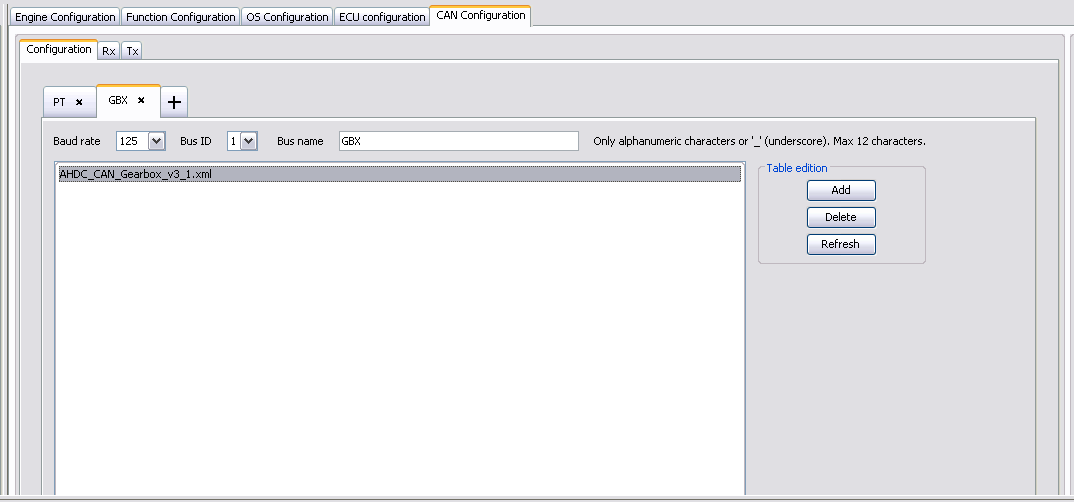
\includegraphics[scale=0.47]{images/ihmcan_conf}}
 \caption{Interface de configuration des bus CAN utilisés par l'application (capture du 17 juin 2015)}
 \label{fig:ihmcan_conf}
\end{figure}

\begin{figure}[h]
  \centering
  \centerline{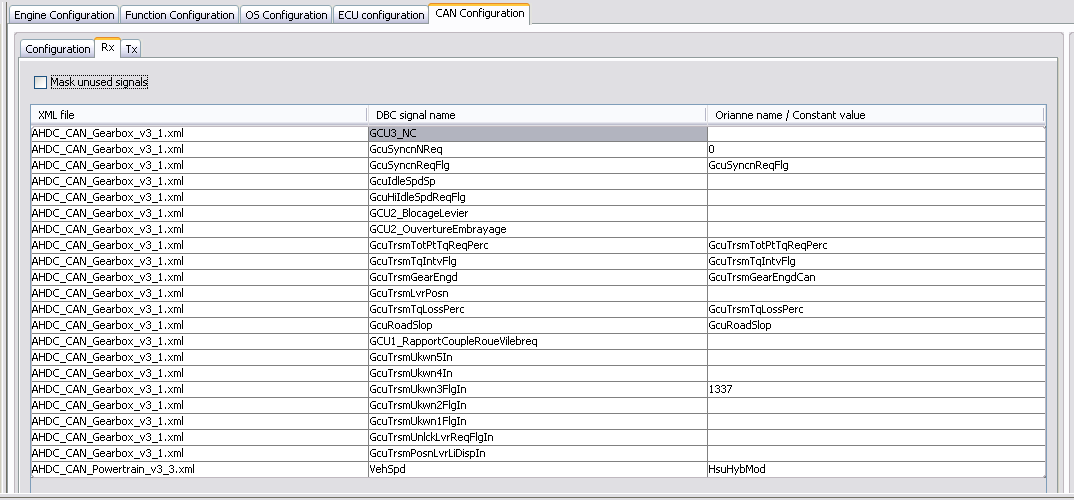
\includegraphics[scale=0.47]{images/ihmcan_signal}}
  \caption{Interface de configuration des signaux CAN (vue des signaux d'entrée, capture du 17 juin 2015)}
  \label{fig:ihmcan_signal}
\end{figure}


\subsection{La partie RTE}
La génération CAN n'est pas le seul outil manquant à la plateforme. Ma
prochaine tâche se tourne vers la partie RTE. Cette partie consiste à définir
les liens entre le code interne à l'ECU (pilotes) et notre application. Pour
cela, on se base sur les différents types d'entrée/sortie fournis par l'ECU. Les
entrées/sorties sont définies dans un fichier de configuration XML propre à
chaque ECU. C'est sur ce fichier là que nous allons nous baser pour la
configuration RTE de l'application.

Du point de vue utilisateur, la configuration RTE se découpe en 3 parties. La
première est la saisie des capteurs et actionneurs, la deuxième est
l'affectation des entrées/sorties de l'ECU aux entrées/sorties des composants
via les capteurs et actionneurs définis précédemment et la troisième est le lien
entre ces entrées/sorties et les variables des modules de l'application. Cela se
traduira par 3 vues différentes dans l'application. Ces 3 étapes permettront de
configurer le générateur qui génèrera les appels aux API pour interfacer les
accès aux variables des capteurs de l'ECU.

Je suis actuellement en cours de conception de l'interface graphique. Comme pour
la partie CAN, elle a vocation à faciliter la configuration de l'application via
des éléments graphiques simples (formulaires, tables, etc.). 
Elle doit s'articuler autour de la configuration possible de l'ECU afin de
fournir le maximum de détails à l'utilisateur tout en restant cohérente avec le
processus de configuration. Par exemple, il faudra que l'utilisateur définisse
les capteurs et actionneurs qu'il souhaite utiliser avant de définir la laison
des données de ces composants avec les paramètres des modules de l'application.
L'IHM doit être construite pour que cet enchaînement de tâche se fasse de la
manière la plus naturelle et la plus intuitive possible.  Il faudra ensuite
développer le générateur basé sur cette IHM qui créera le code relatif à cette
configuration et adaptera la \og glue \fg{} pour prendre en compte ce nouveau
code.


\subsection*{}
La partie CAN est à présent terminée, l'interface est complète et le générateur
fonctionnel. Il est désormais possible de configurer et généré le code relatif à
la communicaiton CAN entièrement depuis l'interface graphique de la plateforme.

La partie RTE est en pleine conception et le développement devrait démarrer
sous peu. Les spécifications ne sont pas figées
encore mais nous avons les premiers prototypes de l'IHM (cf. figure
\ref{fig:rte_conf}). Ils vont nous permettre
de simuler une utilisation de l'outil et de voir les améliorations éventuelles
ou modifications nécessaires dans la spécification pour que l'outil soit agréable
à utiliser mais surtout qu'il permette une configuration poussée et complète de
la partie RTE.

\begin{figure}[h]
  \centering
  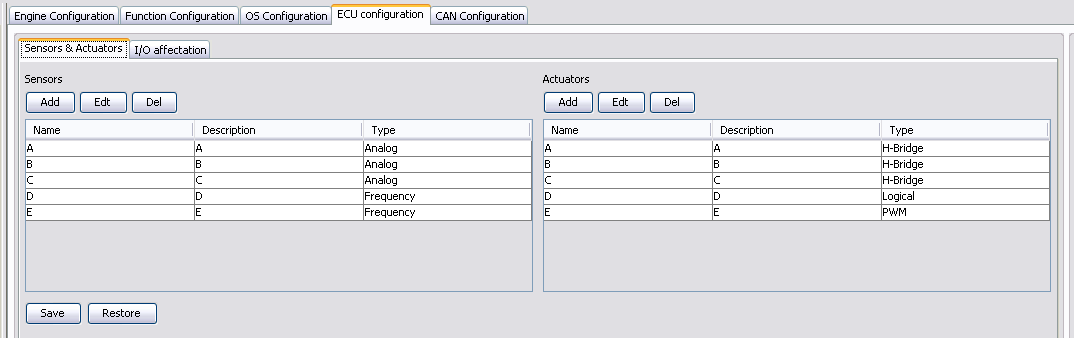
\includegraphics[scale=0.45]{images/rte_conf}
  \caption{Prototype de la configuration des capteurs et actionneurs utilisés. (capture du 17 juin 2015)}
  \label{fig:rte_conf}
\end{figure}


